% ********************************************* %
\section{Problem Description\label{sec:problem}}
% ********************************************* %

HC-Unicamp is a university hospital located in Campinas, São Paulo, Brazil~\citep{hc_unicamp_historia}. 
It is a high-complexity public hospital serving approximately $6.5$ million inhabitants from the Campinas metropolitan area and other regions of Brazil, handling around $500{,}000$ patient cases per year. 
Of these, roughly $10{,}000$ correspond to elective surgical procedures, with the remainder involving outpatient consultations and emergency care~\citep{hc_unicamp_dados}. 
In addition to providing healthcare services, HC-Unicamp operates as a teaching and research hospital, training healthcare professionals and conducting medical and interdisciplinary research.

Elective surgical patients follow a complex, multi-stage care pathway, illustrated in Figure~\ref{fig:patient_flow}, encompassing pre-operative, intra-operative and post-operative phases.
This process begins with waiting-list management, initiated at local medical consultations and coordinated through the regional bed regulation centre, a government agency responsible for regulating hospital access across the region.
Patient entry into HC-Unicamp typically occurs via scheduled outpatient appointments, although some emergency cases subsequently become elective and are incorporated into the same planning process.
Once referred, patients are assigned to waiting lists according to medical subspecialty.
Decisions at this stage directly determine the CMP, influencing waiting times, specialty-level demand balance and the long-term utilisation of operating theatre capacity~\citep{Siqueira2018INTO}.
This decision layer corresponds to the strategic component addressed in this study.

\begin{figure}
    \centering
    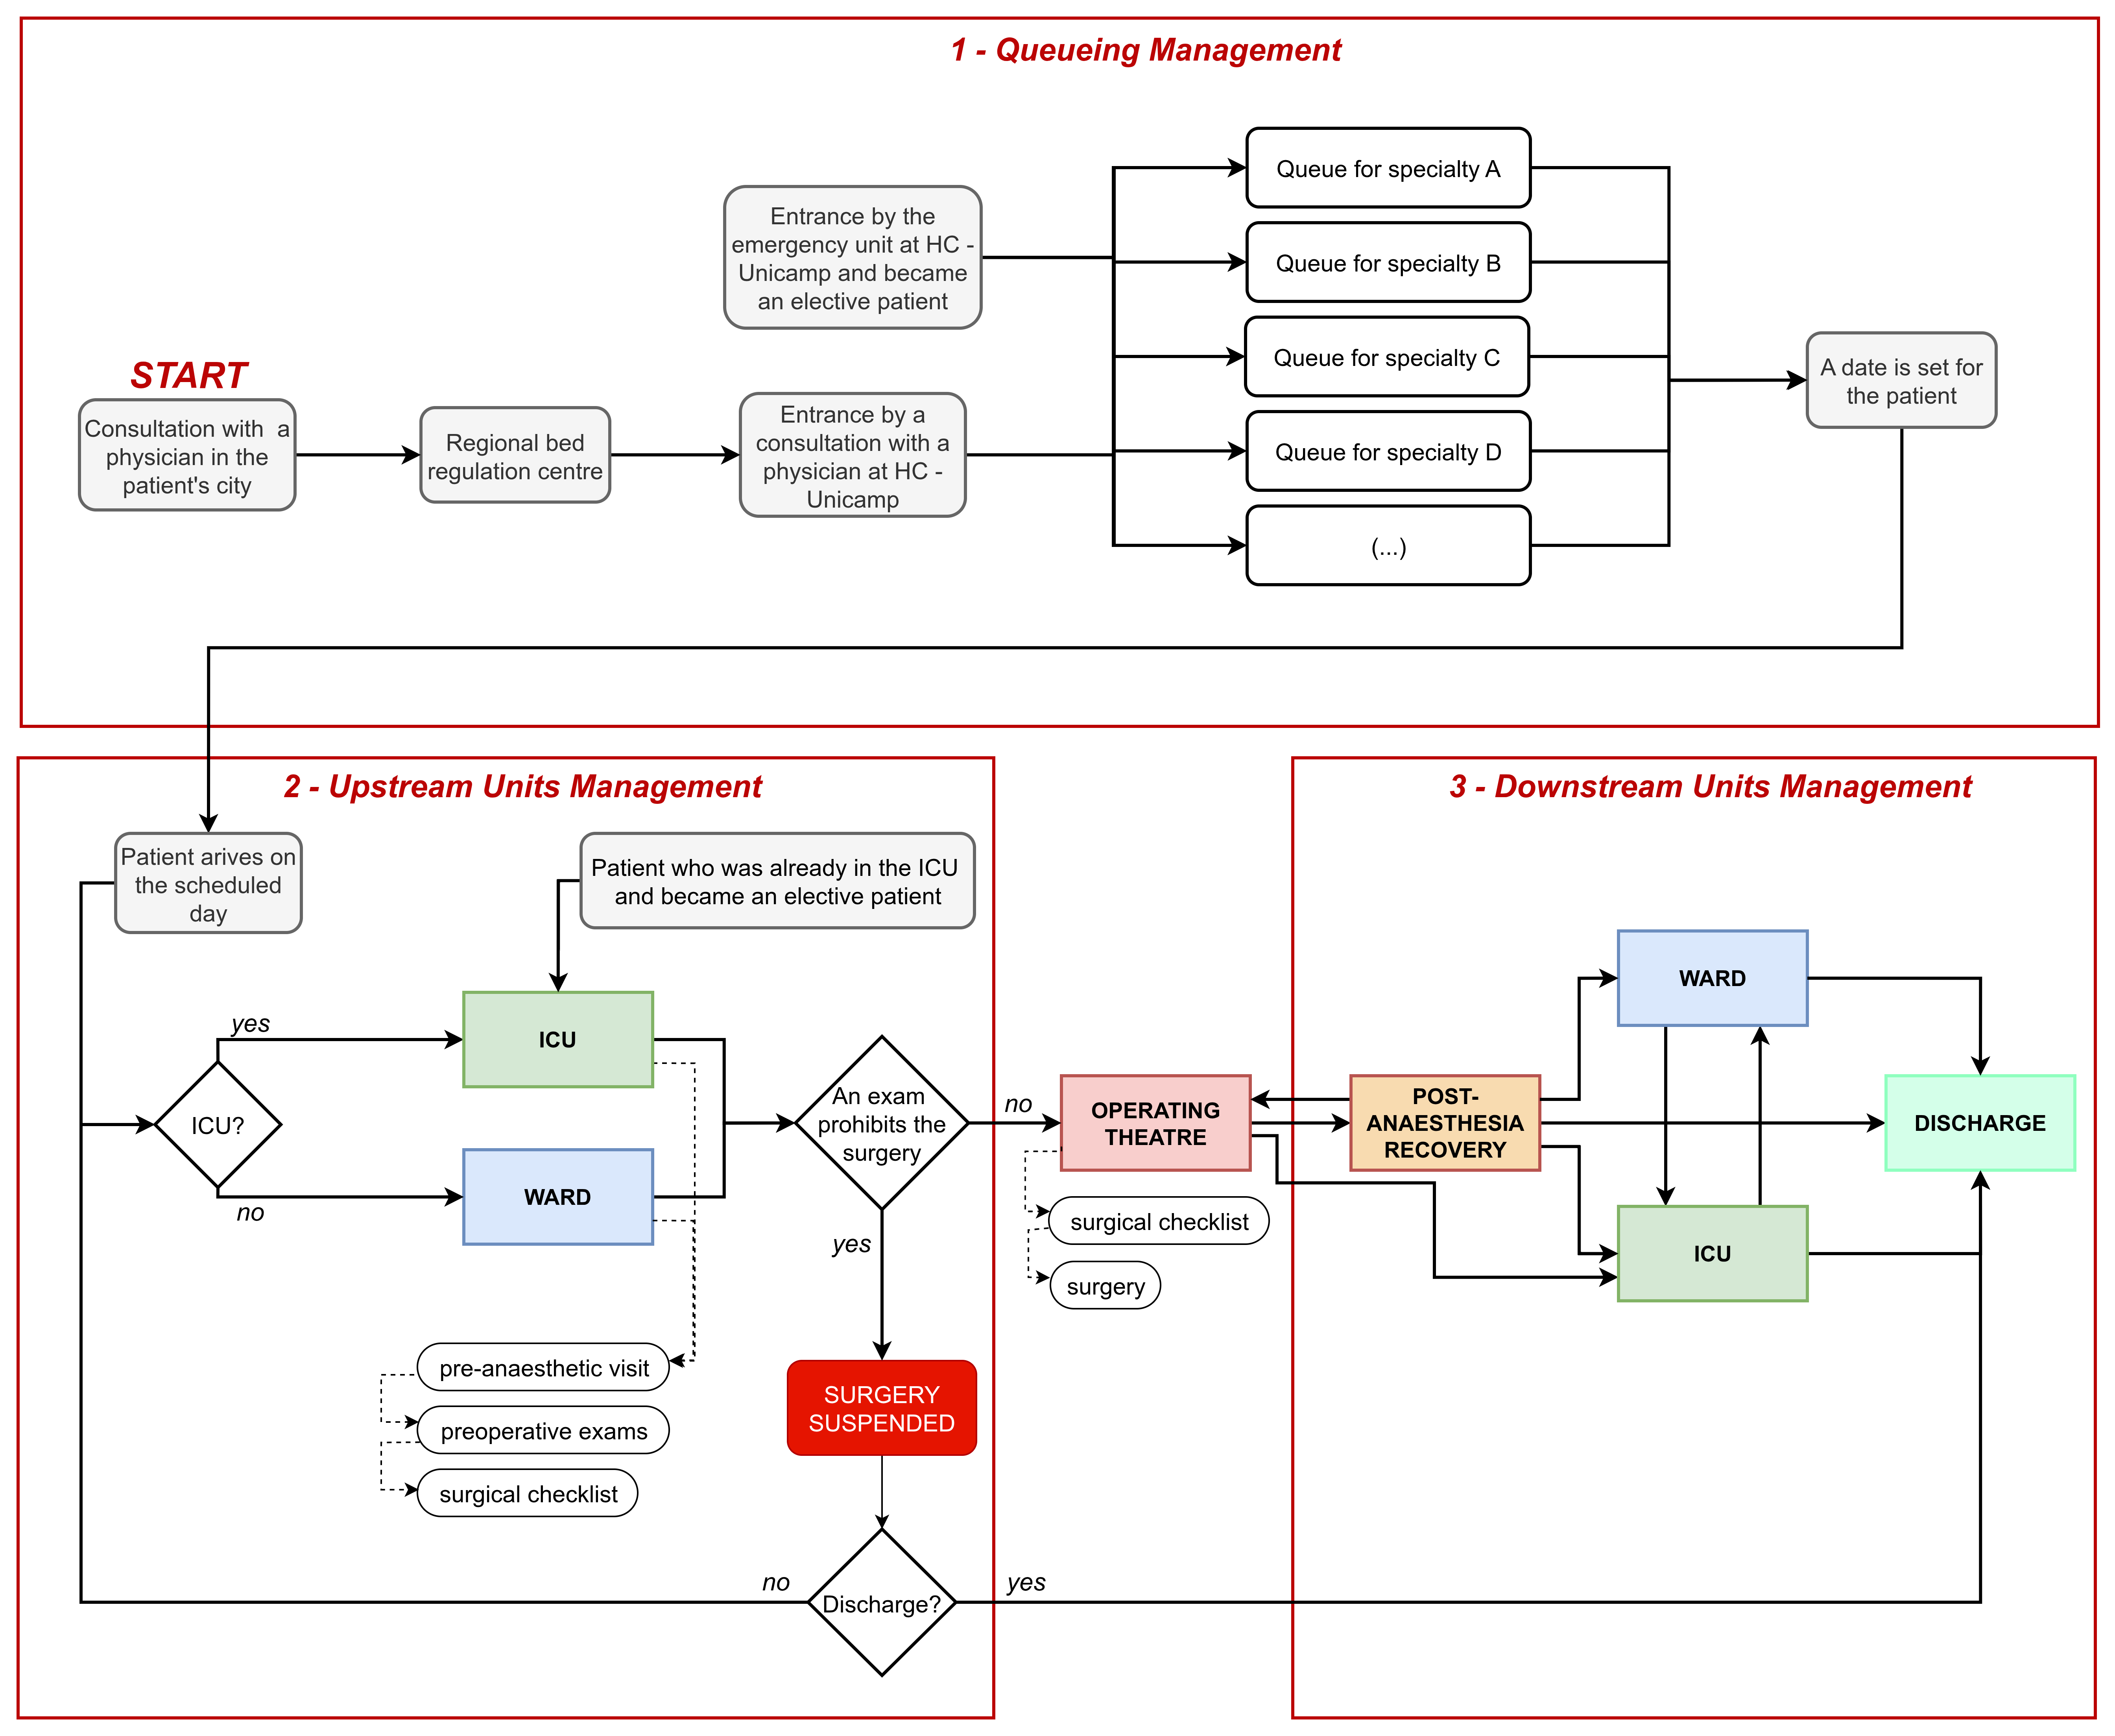
\includegraphics[width=0.9\textwidth]{images/patient_flow.png}
    \caption{Patient flow at HC - Unicamp.\label{fig:patient_flow}}
\end{figure}

On the day of surgery, patients enter the upstream unit management phase, where clinical reassessment is performed.
Depending on clinical requirements, Intensive Care Unit (ICU) support may be needed either pre- or post-operatively, requiring prior bed reservation; otherwise, ward bed availability must be ensured after surgery.
Patients then undergo pre-anaesthetic evaluation, diagnostic tests and surgical safety checks.
If contraindications arise, the procedure is suspended and the patient is either discharged or rescheduled, depending on clinical severity.
If cleared, the patient proceeds to the operating theatre, where the surgical procedure and subsequent theatre cleaning are performed.
In the present study, ward and ICU capacity are sufficient and therefore do not constitute binding constraints, allowing the analysis to focus on waiting-list management, surgery duration uncertainty and operating theatre allocation.

Once in the operating theatre, the patient is managed by a dedicated surgical team and anaesthetist.
This stage includes final safety checks, the surgical procedure itself and post-operative cleaning.
Here, uncertainty in surgery duration plays a central role, as it directly affects idle time, overtime and the risk of cancellations.
Consequently, surgery duration variability has a significant impact on operating theatre utilisation and overall system throughput, motivating its explicit consideration in the proposed framework.

Following surgery, patients are transferred to the Post-Anaesthesia Recovery Unit (PARU), with direct ICU transfer occurring only in exceptional cases.
After stabilisation, patients are admitted to a ward or ICU and subsequently discharged.
Although complications may occasionally require ICU readmission, recovery-unit capacity at HC-Unicamp is sufficient for the planning horizon considered.
This enables the proposed approach to concentrate on integrated waiting-list control, overtime management and operating theatre scheduling, in line with the contributions identified in the literature review.

HC-Unicamp operates $15$ operating theatres dedicated to elective surgeries: $13$ located in the Elective Surgery Centre (ESC) and $2$ in the Ambulatory Surgery Centre (ASC), which operates exclusively during morning shifts.
These theatres are heterogeneous with respect to infrastructure and equipment, leading to compatibility restrictions across medical subspecialties.

Each month, operating theatres must be allocated to $41$ medical subspecialties.
Relevant subsets include: (i) subspecialties requiring two consecutive time blocks; (ii) subspecialties with circumstantial but mandatory demand; (iii) priority subspecialties that take precedence in allocation decisions; and (iv) transplant subspecialties, which impose additional operational constraints.

The planning horizon comprises approximately $20$ working days per month, each divided into two shifts (morning and afternoon), defining $6$-hour time blocks.
Hospital policy assigns each block to a single subspecialty, while allowing the same subspecialty to occupy multiple blocks within the same theatre, provided compatibility conditions are met.
Sequential allocation is therefore permitted (and prefered by hospital managers), enabling a subspecialty assigned to a morning block to also occupy the corresponding afternoon block.

Allocation feasibility depends on the availability of surgical teams and anaesthetists.
A subspecialty can only be assigned to a block if an appropriate team is available on the corresponding day and shift.
Moreover, the number of simultaneous allocations requiring anaesthesia cannot exceed the number of anaesthetists available in each period.
For example, if $15$ anaesthetists are available on a given morning, at most $15$ anaesthesia-dependent procedures may be scheduled concurrently.

\begin{figure}[ht]
    \centering
    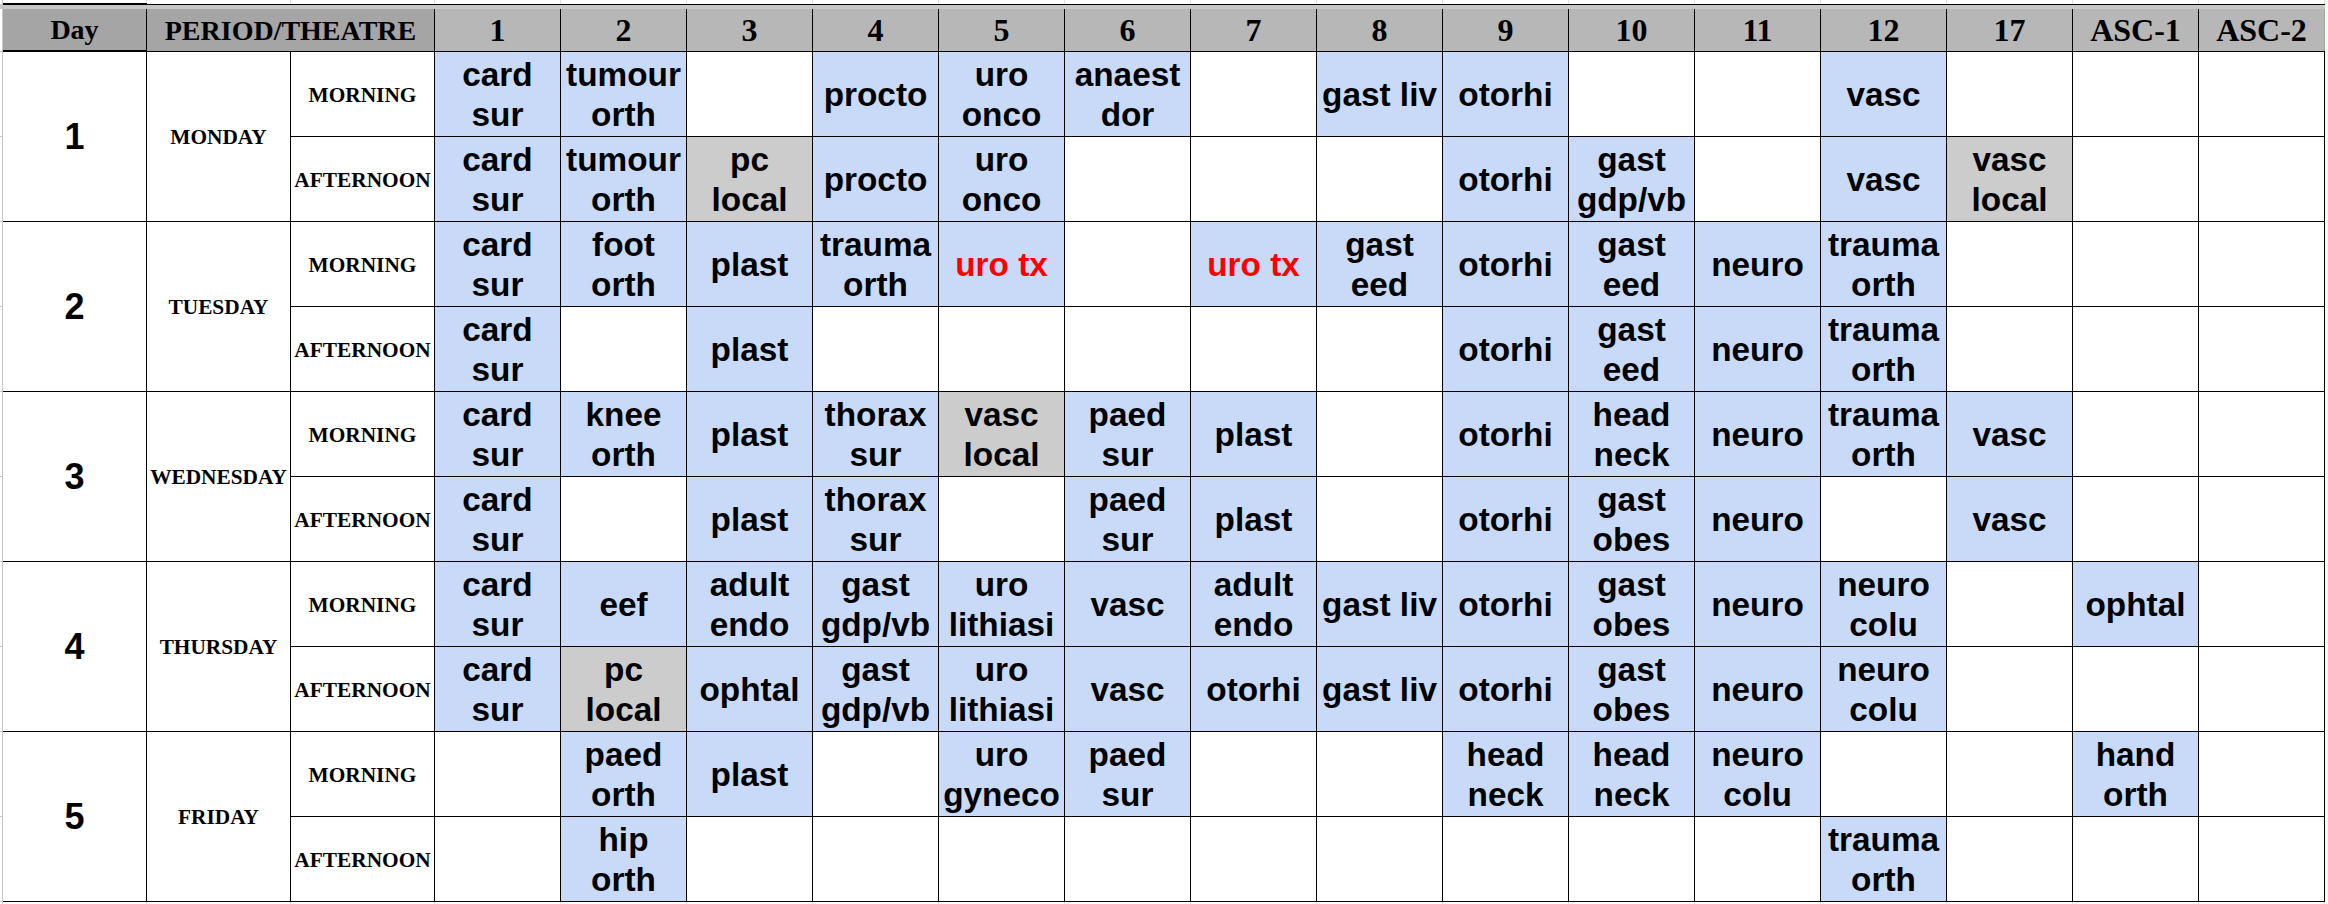
\includegraphics[width=0.9\textwidth]{images/trecho_escala.png}
    \caption{Excerpt from a week's operating theatre schedule.\label{fig:ex_escala}}
\end{figure}

Figure~\ref{fig:ex_escala} presents an excerpt from a weekly operating theatre schedule.
Rows represent time blocks and columns correspond to theatres; subspecialty allocations are colour-coded (blue for procedures requiring anaesthesia and grey otherwise).
Blank cells highlight unallocated slots, reflecting the complexity of the constraint set.
Allocations shown in red correspond to transplant surgeries, which require the simultaneous allocation of two theatres within the same time block.

Historically, schedules such as those shown in Figure~\ref{fig:ex_escala} have been manually constructed using spreadsheets, often requiring more than two full working day.
This manual process is time-consuming and does not guarantee optimality with respect to hospital policies and operational objectives.
Automating the scheduling process therefore reduces administrative burden and enables the generation of optimal or near-optimal solutions under complex constraints.

In this context, proposing an integrated planning framework for elective surgery at HC-Unicamp directly addresses the limitations identified in the literature.
By jointly managing waiting-list dynamics, surgery duration uncertainty and operating theatre allocation, the proposed approach provides a coherent and practically grounded solution capable of satisfying waiting-time requirements while mitigating idle time, overtime and cancellation risks.